\documentclass[a4paper,10pt]{article}
\usepackage[utf8]{inputenc}
\usepackage[a4paper,margin=3.5cm]{geometry} %Sets the page geometry
\usepackage{url}
\usepackage{dirtytalk}
\usepackage{graphicx} % Package for \includegraphics
\usepackage{wrapfig} % Figure wrapping
\usepackage[T1]{fontenc} % Output font encoding for international characters
\setlength{\parskip}{1em} % Set space when paragraphs are used
\usepackage{amssymb}
\usepackage{amsmath}
\usepackage{tcolorbox}
\usepackage{mathtools}
\usepackage{tikz}
\usepackage{amsthm}
\usepackage{caption}
\usepackage{changepage}
\usetikzlibrary{arrows}

% Self Explanatory
\newtheorem{theorem}{Theorem}[section]
\newtheorem{definition}{Definition}[section]
\newtheorem{corollary}{Corollary}[theorem]
\newtheorem{lemma}[theorem]{Lemma}
\newtheorem{exercise}{Exercise}[section]

\theoremstyle{definition} % Set solutions to be bold
\newtheorem*{solution}{Solution}

% Other
\DeclarePairedDelimiter\floor{\lfloor}{\rfloor} %Floor function

% Remove indentation for paragraphs
\setlength{\parindent}{0pt}

\def\changemargin#1#2{\list{}{\rightmargin#2\leftmargin#1}\item[]}
\let\endchangemargin=\endlist 

% Change footnote numbering to numeric style
\renewcommand{\thefootnote}{\arabic{footnote}}


\begin{document}
    \section{Lecture 01}
    This course deals with \emph{abstract mathematical objects}, which
    are defined by the properties they satisfy.

    \textbf{Properties:} defined by propositions/statements which are either true or false. 
    Here are a few examples of propositions:
    \begin{enumerate}
        \item 7 is a prime number.
        \item All natural numbers are even.
        \item All even numbers greater than 2 can be written as the sum of 2 primes.
    \end{enumerate}

    We shall try to define the natural numbers themselves using the properties 
    they satisfy. Let's start with these 2 axioms:

    \begin{tcolorbox}[colback=blue!10!white, colframe=blue!50!black]
    \begin{enumerate}
        \item $0$ is a natural number. \footnotemark
        \item For every natural number $n$, there exists a natural number $n+1$.
    \end{enumerate}
    \end{tcolorbox}
    \footnotetext{Whether we add 0 or not to the set of natural numbers is simply a 
    matter of convention. For this course, it is convenient to add it to the set.}

    The first axiom tells us that there is a starting number (which we call 0), 
    and the second axiom tells us that for every natural number there is a \emph{next} 
    natural number.

    It might be a bit weird to use the addition symbol in our axioms when we haven't 
    even defined numbers yet. Note that this is just a notation; to make it clear
    we can write $next(n)$ instead of $n+1$ to indicate the next natural number. 
    It's best to think of $next(n)$ as a function which just spits out a new natural
    number for each input $n$.

    \textbf{Predicates: }a statement which involves variables, which can take any value
    in some domain. Think of a predicate $P(x)$ as a function which assign true or 
    false to each value x. For example, $P(x)$ could denote \emph{x is the square of
    an integer}.

    There are 3 ways to make a predicate into a proposition:
    \begin{enumerate}
        \item Substitute a constant for x, for example $P(18)$ is a proposition.
        \item $\exists x \ P(x)$: this proposition is true if there is some object
        $a$ for which $P(a)$ is true.
        \item $\forall x \ P(x)$: this proposition is true if $P(x)$ is true for all
        objects x. 
    \end{enumerate}

    Using this notation, we can precisely write our previous 2 axioms for natural numbers:
    \begin{tcolorbox}[colback=blue!10!white, colframe=blue!50!black]
    \begin{enumerate}
        \item $\exists n \ n = 0$
        \item $\forall n \ \exists m \ (m = next(n))$
    \end{enumerate}
    \end{tcolorbox}

    Let's think more about the second axiom. We need to place more restrictions on this 
    \emph{next} function to get our natural numbers. For example, if we allow $next(0) = 0$, 
    our natural numbers just becomes the set $\{0\}$, and it satisfies the axioms we have so far.
    We could also have $next(0) = 1, next(1) = 0$. So one restriction we could think of to
    avoid this is to keep $next(n) \neq 0$ for all $n$.

    \begin{figure}[ht]
    \centering
    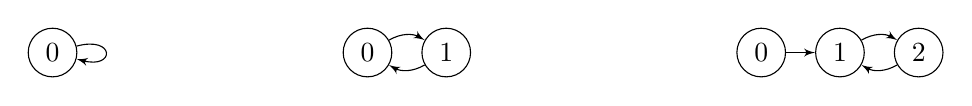
\begin{tikzpicture}
        \tikzset{vertex/.style = {shape=circle,draw,minimum size=1.5em}}
        \tikzset{edge/.style = {->,> = latex'}}
        % vertices
        \node[vertex] (a0) at (0,0) {0};
        \node[vertex] (b0) at (4,0) {0};
        \node[vertex] (b1) at (5,0) {1};
        \node[vertex] (c0) at (9,0) {0};
        \node[vertex] (c1) at (10,0) {1};
        \node[vertex] (c2) at (11,0) {2};
        %edges
        \draw[edge] (a0) to [loop right] ();
        \draw[edge] (b0) to [bend left] (b1);
        \draw[edge] (b1) to [bend left] (b0);
        \draw[edge] (c0) to (c1);
        \draw[edge] (c1) to [bend left] (c2);
        \draw[edge] (c2) to [bend left] (c1);
        
    \end{tikzpicture}

    \caption[Caption for LOF]{Valid number systems\footnotemark\ without any condition
    on \emph{next}}
    \end{figure}
    \footnotetext{It's important to keep in mind what makes one number system different
    from another is how the nodes are linked, it's not about what symbol we keep for each
    node like 0, 1, 2}

    Is this enough? Not really, as we can still think of counterexamples, like
    $next(0) = 1, next(1) = 2, next(2) = 1$. Basically we have ensured that \emph{next}
    doesn't loop back to 0. But we must ensure that it doesn't loop back at all 
    (or even to the same number). How we shall do this is to add the restriction that 
    \emph{next} should not point to a number which has already been mapped to i.e. we make
    it a one-one function. Let's now add these conditions to our axioms:

    \begin{tcolorbox}[colback=blue!10!white, colframe=blue!50!black]
        \begin{enumerate}
            \item $\exists n \ n = 0$
            \item $\forall n \ \exists m \ (m = next(n))$
            \begin{enumerate}
                \item $\forall n \ next(n) \neq 0$
                \item $\forall m \ \forall n \ next(m) = next(n) \implies m = n$
            \end{enumerate}
        \end{enumerate}
    \end{tcolorbox}

    \begin{figure}[ht]
    \centering
    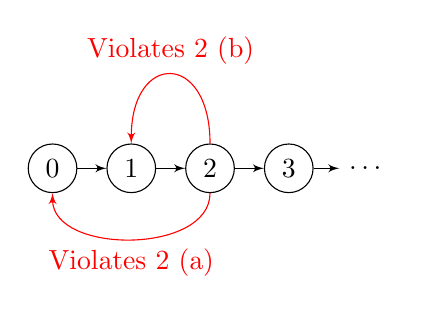
\begin{tikzpicture}
        \tikzset{vertex/.style = {shape=circle,draw,minimum size=1.5em}}
        \tikzset{edge/.style = {->,> = latex'}}
        % vertices
        \node[vertex] (0) at (0,0) {0};
        \node[vertex] (1) at (1,0) {1};
        \node[vertex] (2) at (2,0) {2};
        \node[vertex] (3) at (3,0) {3};
        \node (ellipsis) at (4,0) {\ldots};
        %edges
        \draw[edge] (0) to (1);
        \draw[edge] (1) to (2);
        \draw[edge] (2) to (3);
        \draw[edge] (3) to (ellipsis);
        \draw[red, edge] (2) to [in=90, out=90, looseness=3] node[midway, above] {Violates 2 (b)} (1);
        \draw[red, edge] (2) to [in=270, out=270, looseness=1] node[midway, below] {Violates 2 (a)} (0);
    \end{tikzpicture}
    \caption{Diagrammatic explanation of why \emph{next} always points to a new number}
    \end{figure}

    It turns out our axioms are still not complete. We have ensured that \emph{next}
    always points to a new number, but we haven't really ensured that every natural
    number can be formed by applying \emph{next} to 0 a finite number of times. 
    Here are some counterexamples:
    \begin{enumerate}
        \item $\left\{0, \frac{1}{3}, \frac{2}{3}, \dots\right\}$ where $next(n) = n+1$ 
        \item $[0, \infty)$ where $next(n) = n+1$
    \end{enumerate}
    
    By repeatedly applying \emph{next} to our growing chain, we should end up 
    with the set of all natural numbers. A neat way of stating this is to just
    keep an axiom that induction itself works i.e. if a statement is true for 
    $0, next(0), next(next(0)), \dots$ it must be true for all natural numbers.
    So here is our final set of axioms, which does lead only to our natural numbers:

    \begin{tcolorbox}[colback=blue!10!white, colframe=blue!50!black]
        \begin{enumerate}
            \item $\exists n \ n = 0$
            \item $\forall n \ \exists m \ (m = next(n))$
            \begin{enumerate}
                \item $\forall n \ next(n) \neq 0$
                \item $\forall m \ \forall n \ next(m) = next(n) \implies m = n$
            \end{enumerate}
            \item $[P(0)]  [\forall n \ \{P(n) \implies P(next(n))\}] \implies [\forall n \ P(n)]$
        \end{enumerate}
    \end{tcolorbox}

    \begin{exercise}
        Prove that $\forall n \ next(n) \neq n$. Can we have this statement instead of 
        2 (b) to define natural numbers?
    \end{exercise}
    \begin{solution}
        Proof by induction \\
        Define $P(n)$ to be $\ next(n) \neq n$. $P(0)$ is true from 2 (a). \\
        Also, $next(n) \neq n \implies next(next(n)) \neq next(n)$ as \emph{next} is one-
        one (or contrapositive of 2 (b)). This is basically $P(n) \implies P(next(n))$. \\
        From this we conclude $P(n)$ i.e. $next(n) \neq n$ for all $n$. \\
        This can't be used instead of 2 (b). Counterexample: $next(0) = 1, next(1) = 2, next(2) = 1$.
    \end{solution}

    \begin{exercise}
        Instead of keeping induction as an axiom, we could ensure that there are no other
        starting points for a chain other than 0. This might ensure that all numbers are
        part of the chain starting from 0. 

        Can we replace axiom 3 with the following: \\ 
        $\forall n \ n \neq 0 \iff \exists m \ next(m) = n$
    \end{exercise}
    \begin{solution}
        No, we have a counterexample, take the set \\ 
        $\{0, 1, 2, \dots\} \cup \{\dots, -1.5, -0.5, 0.5, 1.5, \dots\}$ where $next(n)$ is the standard $n+1$. \\
        It satisfies the new set of 3 axioms but aren't equivalent to natural numbers.
    \end{solution}

    \begin{exercise}
        Is there a more concrete way to show that from axiom 3 that all natural numbers
        can be obtained composing $next$ to 0 a finite (including 0) number of times?
    \end{exercise}
    \begin{solution}
        Let $P(n)$ denote $n$ obtained composing \emph(next) to 0 a finite (including 0) 
        number of times. $P(0)$ is obviously true. It's also clear that $P(n) \implies P(next(n))$,
        as if $n$ can be written as $next(next(\dots(next(0))\dots))$, $next(n)$ can also be written
        that way by just composing one more \emph{next} to the expression. 
        This completes our proof.

        Another way we can do this question is proof by contradiction.
        Assume there are some numbers not in the infinite chain starting from 0.
        We define our predicate to be true for values in the infinite chain starting
        from 0, and false for every other value.

        \begin{figure}[ht]
            \centering
            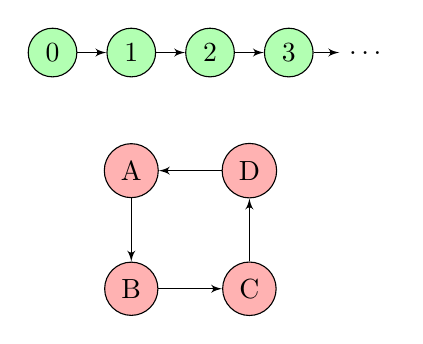
\begin{tikzpicture}
                \tikzset{vertex/.style = {shape=circle,draw,minimum size=1.5em}}
                \tikzset{edge/.style = {->,> = latex'}}
                % vertices
                \node[vertex, fill=green!30] (0) at (0,0) {0};
                \node[vertex, fill=green!30] (1) at (1,0) {1};
                \node[vertex, fill=green!30] (2) at (2,0) {2};
                \node[vertex, fill=green!30] (3) at (3,0) {3};
                \node (ellipsis) at (4,0) {\ldots};

                \node[vertex, fill=red!30] (a) at (1,-1.5) {A};
                \node[vertex, fill=red!30] (b) at (1,-3) {B};
                \node[vertex, fill=red!30] (c) at (2.5,-3) {C};
                \node[vertex, fill=red!30] (d) at (2.5,-1.5) {D};
                %edges
                \draw[edge] (0) to (1);
                \draw[edge] (1) to (2);
                \draw[edge] (2) to (3);
                \draw[edge] (3) to (ellipsis);

                \draw[edge] (a) to (b);
                \draw[edge] (b) to (c);
                \draw[edge] (c) to (d);
                \draw[edge] (d) to (a);
            \end{tikzpicture}
            \caption{Our predicate is true for green cells and false for the red cells}
            \end{figure}
    \end{solution}

    This predicate satisfies $P(0)$ is true. It also satisfies $P(n) \implies P(next(n))$,
    because if $P(n)$ is true only for the green cells, and green cells point to only green cells.
    So induction steps are done, but $P(n) \forall n$ is false. So we have a contradiction.

    \section{Lecture 02}

    To extend our definition, let's define $\leq$ operator.

    \begin{tcolorbox}[colback=blue!10!white, colframe=blue!50!black]
        \begin{enumerate}
            \item $\exists n \ \leq(0, n)$ is true
            \item $\forall n \ \leq(next(n), 0)$
            \item $\forall n \  \forall m \ [\leq(next(n), next(m))\ = \ \leq(n, m)]$
        \end{enumerate}
    \end{tcolorbox}

    \begin{figure}[ht]
    \centering
    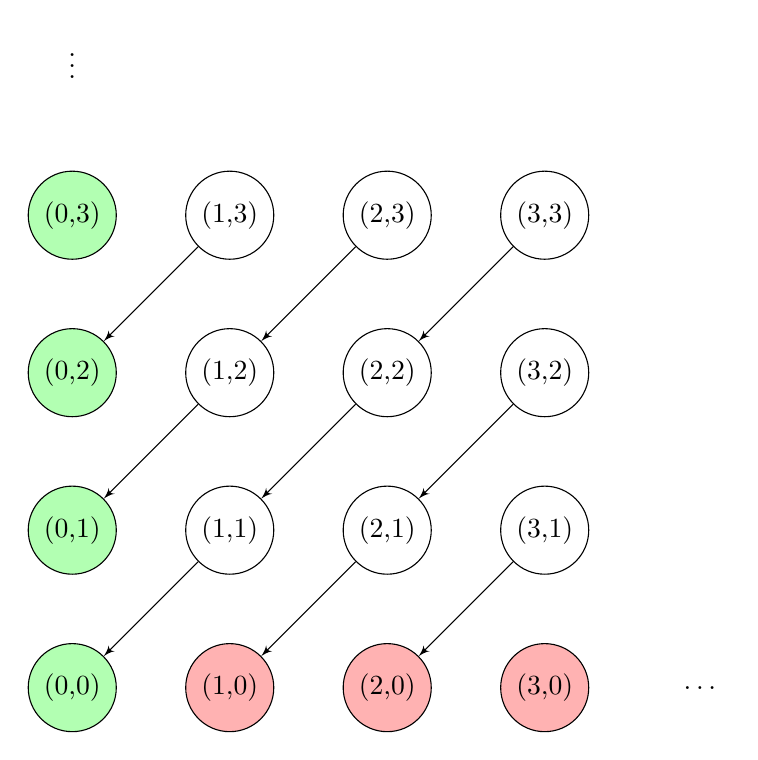
\begin{tikzpicture}
        \tikzset{vertex/.style = {shape=circle,draw,minimum size=1.5em}}
        \tikzset{edge/.style = {->,> = latex'}}

        % vertices
        \foreach \x in {0,...,3}
            \node[vertex, fill=green!30] (0-\x) at (0, 2*\x) {(0,\x)};
        \node (e1) at (0,8) {\vdots};

        \foreach \y in {1,2,3}
            \node[vertex, fill=red!30] (\y-0) at (2*\y,0) {(\y,0)};
        \node (e2) at (8,0) {\ldots};

        \foreach \x in {1,2,3}
            \foreach \y in {1,2,3}
                \node[vertex] (\x-\y) at (2*\x,2*\y) {(\x,\y)};
        

        %edges
        \draw[edge] (1-1) to (0-0);
        \draw[edge] (2-2) to (1-1);
        \draw[edge] (3-3) to (2-2);
        \draw[edge] (2-1) to (1-0);
        \draw[edge] (1-2) to (0-1);
        \draw[edge] (2-3) to (1-2);
        \draw[edge] (3-2) to (2-1);
        \draw[edge] (1-3) to (0-2);
        \draw[edge] (3-1) to (2-0);

    \end{tikzpicture}
    \captionsetup{justification=centering}  % <-- Center the caption
    \caption{Diagrammatic representation of how $\leq$ is defined \\
    $\leq$ is defined as true for green cells, false for red cells \\
    $(A) \rightarrow (B)$ denotes $(A)$ is defined by $(B)$}
    \end{figure}

    From the figure it's intuitive (hopefully) that $\leq(m,n)$ is defined for all $m$ and $n$,
    (3) kind of gives a recursive definition. 
    But how do we prove this? Since our predicate has 2 input variables, there
    is some sort of nested induction.\\
    Take $P(m)$ to be $\forall n \ \leq(m,n)$ is defined. \\
    $P(0)$ is defined from (1).\\
    Now assume $\forall n \ \leq(m,n)$ is defined (which is $P(m)$) \\
    We have to prove $\forall n \ \leq(next(m),n)$ is defined (which is $P(next(m)))$ \\
    The thing is, there's no direct way to proceed from here. It's clear that we somehow
    want to use (3) but we can't as we have $\leq(next(m),n)$ instead of $\leq(next(m),next(n))$.
    How we proceed is we take $Q(n)$ as $\leq(next(m),n)$ is defined, which is want we want to prove
    to complete the induction, and prove $Q(n)$ using induction itself!
    (Note that for the $Q(n)$ statement, $m$ is fixed!)
    $Q(0)$ is true as $\leq (next(m), 0)$ is defined as false. \\
    Now assume $Q(n)$ is true i.e. $\leq(next(m),n)$ is defined. \\
    $Q(next(n))$ is $\leq(next(m),next(n))$ which is $\leq(m,n)$ which is defined, as it is $P(m)$.
    So we proved $\forall n \ Q(n)$, which is the inner induction complete. \\
    This also completes the outer induction.

    \begin{exercise}
        Prove that $\leq(a,b) \ \land \ \leq(b,a) \implies a = b$
    \end{exercise}
    \begin{solution}
        Nested induction on $a$, $b$.\\
        Let $P(a)$ be $\forall b \ \leq(a,b) \ \land \ \leq(b,a) \implies a = b$ \\
        First we need to show that $P(0)$ is true. $\leq(0,b)$ is always true, also
        we can see that $\leq(b,0)$ is true implies $b$ is $0$ as if it's not the case,
        $b$ can be written as $next(k)$ and $\leq(next(k),0)$ is false. \\
        Now for the induction, assume $\leq(a,b) \ \land \ \leq(b,a) \implies a = b$ \quad ($\ast$)\\
        To prove: $\leq(next(a),b) \ \land \ \leq(b,next(a)) \implies next(a) = b$ \\
        Nested induction now, take the above as $P(b)$. 
        \begin{adjustwidth}{2cm}{0cm}
            $P(0)$ is a vacuous truth as $\leq(next(a),0)$ is false. \\
            Now assuming $P(b)$ we have to prove $P(next(b))$, which is \\
            $\leq(next(a),next(b)) \ \land \ \leq(next(b),next(a)) \implies next(a) = next(b)$ \\
            But this is just equivalent to ($\ast$), as LHS of the implication can be 
            simplified by the recursive definition of $\leq$ and RHS of the implication can be 
            simplified with one-oneness of \emph{next}. \\
            So inner induction is complete.
        \end{adjustwidth}
        This also completes outer induction as we have proved $\forall b \ P(b)$
    \end{solution}

    \begin{exercise}
        Prove that $\leq(a,b) \ \land \ \leq(b,c) \implies \leq(a,c)$
    \end{exercise}
    \begin{solution}
        Nested induction again\dots \\
        Let $P(a)$: $\forall b \ \forall c \ \leq(a,b) \ \land \ \leq(b,c) \ \implies \ \leq(a,c)$ \\
        $P(0)$ is true as RHS of implication is always true. \\
        Now assume $P(a)$: $\forall b \ \forall c \ \leq(a,b) \ \land \ \leq(b,c) \ \implies \ \leq(a,c)$ \quad $(\ast)$ \\
        To prove $P(next(a))$: $\forall b \ \forall c \ \leq(next(a),b) \ \land \ \leq(b,c) \ \implies \ \leq(next(a),c)$
        \begin{adjustwidth}{1cm}{0cm}
            Let $Q(b)$: $\forall c \ \leq(next(a),b) \ \land \ \leq(b,c) \ \implies \ \leq(next(a),c)$ \\
            $Q(0)$ is true as first term of LHS of implication is false. \\
            Now assuming $Q(b)$ we have to prove $Q(next(b))$, which is: \\
            $\forall c \ \leq(next(a),next(b)) \ \land \ \leq(next(b),c) \ \implies \ \leq(next(a),c)$
            \begin{adjustwidth}{1cm}{0cm}
                Let $R(c)$: $\leq(next(a),next(b)) \ \land \ \leq(next(b),c) \ \implies \ \leq(next(a),c)$ \\
                $R(0)$ is true as second term of LHS of implication is false. \\
                Now assume $R(c)$, we have to prove $R(next(c))$, which is: \\
                $\leq(next(a),next(b)) \ \land \ \leq(next(b),next(c)) \ \implies \ \leq(next(a),next(c))$ \\
                This can be reduced by the recursive definition to ($\ast$) which is assumed as true.
            \end{adjustwidth} 
        \end{adjustwidth}
        That completes all the induction layers.
    \end{solution}

    \begin{exercise}
        Prove that $\leq(a, next(b)) \ \implies \ [\leq(a,b)] \lor [a=next(b)]$ \\
        Use this to prove $[\leq(a,b)] \land [\leq(b,next(a))] \ \implies \ [b=a] \lor [b=next(a)]$
    \end{exercise}
    \begin{solution}
        Let $P(a)$: $\forall b \ \leq(a, next(b)) \ \implies \ [\leq(a,b)] \lor [a=next(b)]$ \\
        $P(0)$ is true as $\leq(0,b)$ is always true. \\
        Now assuming $P(a)$, we have to prove $P(next(a))$.
        \begin{adjustwidth}{1cm}{0cm}
            Let $Q(b)$: $\leq(next(a), next(b)) \ \implies \ [\leq(next(a),b)] \lor [next(a)=next(b)]$ \\
            $Q(0)$: $\leq(a, 1) \ \implies \ [\leq(a,0)] \lor [a=1]$ \\
            We can first simplify $\leq(a,0)$ to $a=0$ using Exercise 2.1's property. \\
            Let's take $Q(0)$ as $R(a)$ and prove that using induction.
            \newpage
            \begin{adjustwidth}{1cm}{0cm}
                $R(0)$ is true as $\leq(a,0)$ is true. \\
                Now assuming $R(a)$ we have to prove $R(next(a))$. \\
                $\leq(next(a),1) \implies \leq(a,0) \implies a=0 \implies next(a)=1$ so $R(next(a))$ is true \\
                So $R(a)$ is true for all a.
            \end{adjustwidth}
            Now assuming $Q(b)$ we have to prove $Q(next(b))$ \\
            But that can be reduced to just $P(a)$ which is assumed as true. \\
            This completes the induction.
        \end{adjustwidth}
        
        For the second part, we know : \\
        $\leq(b, next(a)) \ \implies \ [\leq(b, a)] \lor [b = next(a)]$ \\
        And if $\leq(b, a)$ since we also know $\leq(a, b)$, $b = a$
    \end{solution}

    We now define the addition function $add(m, n)$: 
    \begin{tcolorbox}[colback=blue!10!white, colframe=blue!50!black]
        \begin{enumerate}
            \item $add(0, m) = m$
            \item $add(next(n), m) = next(add(n, m))$
        \end{enumerate}
    \end{tcolorbox}
    It's not too hard to show this sufficiently defines addition by taking $P(n)$ as
    [$add(n, m)$ is defined] and using induction.

    \begin{exercise}
        Prove that $add(add(a,b), c) = add(a, add(b,c))$ which is the associative property
    \end{exercise}
    \begin{solution}
        We can somehow avoid nested induction for once :) \\
        Let $P(a)$ be $\forall b \ \forall c \ add(add(a,b), c) = add(a, add(b,c))$ \\
        To prove $P(0)$, $LHS = add(add(0,b), c) = add(b,c)$ and $RHS = add(0, add(b,c)) = add(b,c)$ \\
        To prove $P(next(a))$, assuming $P(a)$ is true: \\
        $LHS = add(add(next(a),b), c) = add(next(add(a,b)), c) = next(add(add(a,b), c))$ \\
        $RHS = add(next(a), add(b,c)) = next(add(a, add(b,c)))$ \\
        And from $P(a)$ these both are equal.
    \end{solution}

    \begin{exercise}
        Prove that $add(a,b) = add(b,a)$ which is the commutative property
    \end{exercise}
    \begin{solution}
        Lot of induction again :( \\
        Let $P(a)$ be $\forall b \ add(a,b) = add(b,a)$ \\
        $P(0)$ is $\forall b \ add(0,b) = b = add(b,0)$, this itself has to be done by induction on b. \\
        Now assume $P(a)$ which is $\forall b \ add(a,b) = add(b,a)$ \quad ($\ast$) \\
        Basically whenever we have $a$ in the add function we can swap stuff. \\
        To prove: $P(next(a))$ which is $\forall b \ add(next(a),b) = add(b,next(a))$ \\
        We can simplify LHS a bit: $add(next(a),b) = next(add(a,b)) = next(add(b,a))$ from ($\ast$)
        \begin{adjustwidth}{1cm}{0cm}
            Let $Q(b)$ be $add(b, next(a)) = next(add(b,a))$ \quad ($\ast\ast$) \\
            $Q(0)$ is true as we get $LHS = RHS = next(a)$ \\
            Now assume $Q(b)$, we have to prove $Q(next(b))$ \\
            LHS for this is $add(next(b), next(a)) = next(add(b, next(a)))$ \\
            RHS is $next(add(next(b,a)))$ which is $next(next(add(b,a)))$ \\
            And from ($\ast\ast$) both of these are equal
        \end{adjustwidth}
        This completes all the induction.
    \end{solution}

    \newpage
    \begin{exercise}
        Prove that $\leq(a,b) \ \implies \ \exists c$ such that $add(a,c) = b$
    \end{exercise}
    \begin{solution}
        Let $P(a)$ be the above statement for all $b$. \\
        $P(0)$ is true as $c = b$ works. \\ 
        Now assume $P(a)$ is true. \quad ($\ast$) \\
        We have to prove $P(next(a))$, take this as $Q(b)$.
        \begin{adjustwidth}{1cm}{0cm}
            $Q(0)$ is vacuously true as $\leq(next(a), 0)$ is false. \\
            Now assuming $Q(b)$ we have to prove $Q(next(b))$ \\
            $\leq(next(a), next(b)) \ \implies \ \leq(a,b)$ \\
            So from ($\ast$) we know $\exists c$ such that $add(a,c) = b$ \\
            But this also implies $add(next(a), c) = next(b)$ \\
            This proves $Q(next(b))$ which completes all the induction.
        \end{adjustwidth}
    \end{solution}

    \section{Lecture 03}
    Rather than using induction, there's an equivalent way to define natural numbers called
    well-ordering principle. Here are the axioms:

    \begin{tcolorbox}[colback=blue!10!white, colframe=blue!50!black]
        \begin{enumerate}
            \item $\exists n \ n = 0$
            \item $\forall n \ \exists m \ (m = next(n))$
            \begin{enumerate}
                \item $\forall n \ next(n) \neq 0$
                \item $\forall m \ \forall n \ next(m) = next(n) \implies m = n$
                \item $\forall n \ [n = 0] \lor [\exists m \ n = next(m)]$
            \end{enumerate}
            \item $\exists \ \leq$
            \begin{enumerate}
                \item $\forall n \ \lnot \leq(next(n), n)$
                \item $\forall P \ [(\exists n \ P(n)) \ \implies \ \exists n \ (P(n) \ \land \ \forall m(P(m) \implies n \leq m))]$
            \end{enumerate}
        \end{enumerate}
    \end{tcolorbox}

    This might look like it's very complicated using predicate logic, so let's try to see
    what all this means. So the beginning is pretty much like the previous axioms, but 2(c)
    is new. It basically says every number is either 0 or is the \emph{next} of some other number.
    We'll later see how this axiom helps in proving induction itself.

    What does the third axiom say? It says there exists \textbf{some} predicate $\leq$, which 
    is not necessarily the $\leq$ we saw in Lecture 02. But anyways there's some predicate
    $\leq$ which `orders' the natural numbers. What exactly do we mean by that? 3(a) says
    \emph{next} of any number is greater than it. 3(b) says that for all predicates $P$, if
    there is at least one number for which $P$ is true, there will a `smallest' number for
    which it is true. How we write this formally is that there is some $n$ for which $P(n)$ is
    true and for every other $m$ for which it is true, $n \leq m$.

    Let's see how induction is true from these axioms. We prove induction by contradiction.
    Assume there is a predicate $P$ such that $P(0)$ is true, and $P(n) \implies P(next(n))$.
    But $\forall n \ P(n)$ is false, that is there's some $n$ for which $\lnot P(n)$ is true.
    Let the smallest $n$ that satisfies this be $n_0$ (we're using 3(b) here).
    $n_0 \neq 0$ as $P(0)$ is true. So from 2(c) there's $m$ such that $next(m) = n_0$.
    Is $P(m)$ true? If it was, $P(m) \implies P(next(m))$, which would make $P(n_0)$ true.
    \newpage
    So $P(m)$ is false, but haven't we just found a number smaller than $n_0$ which satisfies
    $\lnot P(n)$, which contradicts well-ordering? From 3(a) we know $\leq(n, m)$ is false\footnote
    {Without 3(a) we can't actually conclude this, remember this isn't our familiar
    $\leq$, this is just an arbitrary predicate which satisfies well-ordering}.
    So from 3(b) we can get our contradiction, but remember the predicate we are using is 
    $\lnot P$ instead of $P$. We have $n$ such that $\lnot P(n)$, so 3(b) guarantees
    there exists $n_0$ such that $\lnot P(n)$ is true, and for all other $m$ that
    satisfies $\lnot P(n)$, $\leq(n,m)$. So 3(a) and 3(b) form our contradiction.

    \begin{exercise}
        We have seen how 2(c) was used in proving induction, but maybe even without it
        maybe we get only natural numbers? Is there a number system which isn't natural numbers
        but satisfies everything except 2(c)?
    \end{exercise}

    \begin{solution}
        In fact there are.
        $\{0, 1, 2, \dots, \omega, \omega+1, \omega+2, \dots\}$ form a number system. \\
        Here $\leq$ is what you'd expect it to be, the numbers are arranged in order 
        already, and $\omega$ is greater than all the natural numbers. 
        $\leq$ satisfies all the properties it needs to, even things like 
        the transitive property. But 2(c) forbids such things are there is no $n$
        such that $next(n) = \omega$. These are actually called the ordinal numbers.
        Thing is, we get many useful number systems if we make small changes to our axioms,
        for example if we remove $next(n) \neq 0$ we get modular arithmetic.

        \begin{figure}[ht]
            \centering
            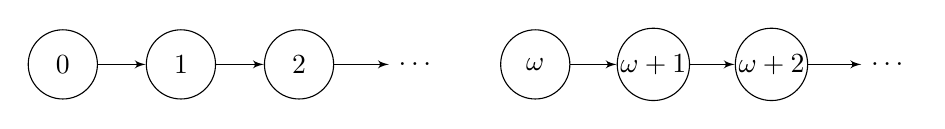
\begin{tikzpicture}
                \tikzset{vertex/.style = {shape=circle,draw,minimum size=2.5em}}
                \tikzset{edge/.style = {->,> = latex'}}
                % vertices
                \node[vertex] (0) at (0,0) {0};
                \node[vertex] (1) at (1.5,0) {1};
                \node[vertex] (2) at (3,0) {2};
                \node (e1) at (4.5,0) {\ldots};
                \node[vertex, inner sep=0.5pt] (w) at (6,0) {$\omega$};
                \node[vertex, inner sep=0.5pt] (w1) at (7.5,0) {$\omega + 1$};
                \node[vertex, inner sep=0.5pt] (w2) at (9,0) {$\omega + 2$};
                \node (e2) at (10.5,0) {\ldots};

                %edges
                \draw[edge] (0) to (1);
                \draw[edge] (1) to (2);
                \draw[edge] (2) to (e1);
                \draw[edge] (w) to (w1);
                \draw[edge] (w1) to (w2);
                \draw[edge] (w2) to (e2);
            \end{tikzpicture}
            \caption{Valid number system without 2(c)}
        \end{figure}        

    \end{solution}
\end{document}